\documentclass[letterpaper,11pt]{article}

 %\documentclass[letterpaper,onepage,openright,titlepage,openany,oneside,11pt]{book}
\usepackage[T1]{fontenc}
\usepackage[latin1]{inputenc}
\usepackage{amsmath}
\usepackage{amsthm}
\usepackage{amsfonts}
\usepackage{amssymb}
\usepackage[spanish]{babel}
\usepackage[latin1]{inputenc}
\usepackage{graphicx}
\usepackage{amsmath}
\usepackage{dsfont} % colocar los numeros r
\usepackage{float}
\usepackage{fancyhdr}
\usepackage{anysize}
\usepackage{booktabs}
\usepackage{multirow}
\usepackage{titlesec}
\usepackage{enumerate}
\usepackage{verbatim}
\newtheorem{theorem}{Theorem}
\newtheorem{definition}{Definition}

\renewcommand{\baselinestretch}{1.5} % 1.5 denotes double spacing. Changing it will change the spacing

\setlength{\parindent}{0in} 


%%%%%%%%%%
\marginsize {3.8cm}{3.5cm}{4cm}{1.6cm}
\setlength{\paperheight}{24cm} \setlength{\paperwidth}{18cm}
\newtheorem{thm}{Teorema}[section]
\newtheorem{cor}[thm]{Corolario}
\newtheorem{defn}[thm]{Definici\'{o}n}
\newtheorem{ej}[thm]{Ejemplo}
\newtheorem{lem}[thm]{Lema}
\newtheorem{prop}[thm]{Proposici\'{o}n}
\def\bibname{Referencias}
\renewcommand{\contentsname}{Contenido}
\renewcommand{\baselinestretch}{1.1} 
 \renewcommand{\labelenumi}{\Roman{enumi}.} %interlineado
\def\chaptername{Cap\'{\i}tulo }
\decimalpoint

\bibliographystyle{apalike}

\begin{document}
%\thispagestyle{fancy} % All pages have headers and footers
\renewcommand{\tablename}{Tabla}
\fancyhf{} % delete current setting for header and footer
\fancyhead[LE,RO]{\bfseries\thepage}
%
\fancyhead[LO]{\bfseries\rightmark}%
\fancyhead[RO,LE]{\thepage} % N�meros de p�gina en las esquinas de los encabezados
\title{Confiabilidad Bayesiana en Transformadores de Instrumento}
%\author{Alma Maldonado Santiago   Andres Christen         Enrique Villa}
\author{\makebox[.9\textwidth]{Alma Maldonado Santiago\footnote{CIO, Centro de Investigaciones en \'Optica, Le�n Guanajuato, M�xico.}}\\ \and Andres Christen\footnote{CIMAT, Centro de Investigaci\'on en Mat\'ematicas, Guanajuato, M�xico} \\ \and Enrique Villa}
\maketitle
\abstract{\noindent En el 2006 los transformadores de instrumento en las  sub\'areas de Coatzacoalcos y Temascal (Veracruz), observaron un n\'umero inusualmente elevado de fallas, lo que condujo a la necesidad de estudiar la confiabilidad de los transformadores. Se deseaba pronosticar el n\'umero de fallas de sus equipos  por a\~no.
\noindent En este trabajo se dise\~na una metodolog\'ia para la construcci\'on de un plan \'optimo de almacenamiento de transformadores, esta construcci\'on se realiza desde un enfoque bayesiano. Haciendo uso de una funci\'on de p\'erdida que ser\'a definida en un contexto, que permita minimizar los costos del almac\'en.}\\[0.1cm]


{\bf \noindent Palabras claves: Transformadores, confiabilidad, Estad\'istica Bayesiana, Funci\'on de utilidad, t-walk, optimizaci\'on, simulaci\'on.}
\section{Introducci\'on}

%En el estudio realizado por el CIMAT, se hizo un an\'alisis de los datos disponibles, empezando por un an\'alisis exploratorio. Posteriormente realizaron distintas comparaciones por tipo, estatus y marca de los transformadores, para  finalmente centrarse en el estudio de los transformadores con m\'as fallas, que resultaron ser los transformadores de corriente. \\[0.1cm]
\noindent Los transformadores de instrumento son herramientas costosas y dif\'iciles de transportar. La mayor\'ia de las empresas que fabrican este tipo de transformadores lo hacen bajo pedido y se tardan un tiempo considerable en cumplirlo. Su abastecimiento resulta una tarea a optimizar, debido a los costos que pueden minimizarse, como transporte y el costo del almacenamiento mismo, cuando no se usaron los aparatos. Sin embargo esta optimizaci\'on, debe ser tal que no permita que la empresa se quede sin transformadores puesto que esto implicar\'ia un costo  por no poder cobrar el servicio.
\begin{table}[h!]\small
\begin{center}
\caption {\bf Tiempos de vida de transformadores de corriente, $t_i$ (meses), $e_i=1$ indica un dato censurado, $e_i=0$ es un dato no censurado.\label{uno}}
\begin{tabular}{ccc|ccc|ccc|ccc}
\toprule[0.6mm]
$i$	&	$t_i$	&	$t_i$	&	$i$	&	$t_i$	&$e_i$	&	$i$	&	$t_i$	&	$e_i$	&	$i$	&	$t_i$	&	$e_i$	\\
\toprule[0.6mm]
1	&	8	&	1	&	36	&	107	&	0	&	106	&	272	&	1	&	141	&	308	&	0	\\
2	&	8	&	1	&	37	&	116	&	1	&	107	&	272	&	1	&	142	&	308	&	0	\\
3	&	8	&	1	&	38	&	119	&	0	&	108	&	272	&	1	&	143	&	308	&	1	\\
4	&	8	&	1	&	39	&	119	&	0	&	109	&	272	&	1	&	144	&	308	&	1	\\
5	&	8	&	1	&	40	&	139	&	0	&	110	&	272	&	1	&	145	&	308	&	1	\\
6	&	20	&	1	&	41	&	140	&	0	&	111	&	274	&	0	&	146	&	308	&	1	\\
7	&	20	&	1	&	42	&	144	&	0	&	112	&	274	&	0	&	147	&	308	&	1	\\
8	&	20	&	1	&	43	&	146	&	0	&	113	&	274	&	0	&	148	&	308	&	1	\\
9	&	20	&	1	&	44	&	146	&	0	&	114	&	275	&	0	&	149	&	308	&	1	\\
10	&	32	&	1	&	45	&	152	&	1	&	115	&	275	&	0	&	150	&	308	&	1	\\
11	&	32	&	1	&	46	&	159	&	0	&	116	&	275	&	0	&	151	&	308	&	1	\\
12	&	32	&	1	&	47	&	159	&	0	&	117	&	276	&	0	&	152	&	308	&	1	\\
13	&	32	&	1	&	48	&	159	&	0	&	118	&	281	&	0	&	153	&	308	&	1	\\
14	&	32	&	1	&	49	&	160	&	0	&	119	&	281	&	0	&	154	&	308	&	1	\\
15	&	32	&	1	&	50	&	161	&	0	&	120	&	284	&	0	&	155	&	308	&	1	\\
16	&	32	&	1	&	51	&	164	&	1	&	121	&	284	&	0	&	156	&	308	&	1	\\
17	&	56	&	1	&	52	&	167	&	0	&	122	&	284	&	0	&	157	&	308	&	1	\\
18	&	80	&	1	&	53	&	172	&	0	&	123	&	284	&	0	&	158	&	308	&	1	\\
19	&	80	&	1	&	54	&	172	&	0	&	124	&	286	&	0	&	159	&	308	&	1	\\
20	&	80	&	1	&	55	&	176	&	1	&	125	&	286	&	0	&	160	&	308	&	1	\\
21	&	80	&	1	&	56	&	183	&	0	&	126	&	286	&	0	&	161	&	308	&	1	\\
22	&	80	&	1	&	57	&	188	&	1	&	127	&	287	&	0	&	162	&	308	&	1	\\
23	&	80	&	1	&	58	&	203	&	0	&	128	&	288	&	0	&	163	&	308	&	1	\\
24	&	80	&	1	&	59	&	205	&	0	&	129	&	288	&	0	&	164	&	308	&	1	\\
25	&	80	&	1	&	60	&	214	&	0	&	130	&	288	&	0	&	165	&	308	&	1	\\
26	&	80	&	1	&	61	&	214	&	0	&	131	&	288	&	0	&	166	&	308	&	1	\\
27	&	80	&	1	&	62	&	215	&	0	&	132	&	296	&	1	&	167	&	308	&	1	\\
28	&	80	&	1	&	63	&	216	&	0	&	133	&	296	&	1	&	168	&	308	&	1	\\
29	&	80	&	1	&	64	&	216	&	0	&	134	&	296	&	1	&	169	&	308	&	1	\\
30	&	80	&	1	&	65	&	216	&	0	&	135	&	296	&	1	&	170	&	308	&	1	\\
31	&	80	&	1	&	66	&	218	&	0	&	136	&	298	&	0	&	171	&	308	&	1	\\
32	&	80	&	1	&	67	&	218	&	0	&	137	&	299	&	0	&	172	&	308	&	1	\\
33	&	94	&	0	&	68	&	218	&	0	&	138	&	300	&	0	&	173	&	308	&	1	\\
34	&	94	&	0	&	69	&	225	&	0	&	139	&	308	&	0	&		&		&		\\
35	&	94	&	0	&	70	&	225	&	0	&	140	&	308	&	0	&		&		&		\\
\bottomrule[0.6mm]
\end{tabular}
\end{center}
\end{table}



\noindent Los elementos disponibles dentro del estudio, 
es una base de datos de transformadores de instrumento de corriente en las sub\'areas de  
Coatzacoalcos y Temascal. Se disponen de sus tiempos de vida  a lo largo de 26 a\~nos hasta el 2006, con datos censurados y no 
censurados. 

\noindent Los datos se muestran en la Tabla \ref{uno}, representados de la siguiente manera, 
$(\underline{t},\underline{e})=\{t_i,e_i\}^n_{i=1}$, donde $e_i=1$ indica que 
el transformador $i$ aun sigui\'o en 
operaci\'on al final de 2006, lo que implica que  es un dato censurado por la derecha. Mientras que $e_i=0$, se refiere a un valor no censurado. De estudios 
anteriores realizados por el CIMAT, los tiempos de vida son modelados adecuadamente 
por medio de una 
distribuci\'on Weibull. La funci\'on de Verosimilitud bajo 
este modelo se expresa 
de la siguiente manera:
\begin{eqnarray}\label{tiempos}
f(\underline{t}|\underline{e},\beta,\eta)&=& \prod_{e_i=0}\frac{\beta}{\eta}\left(\frac{t_i}{\eta}\right)^{\beta-1}\exp \left\{-\left(\frac{t_i}{\eta}\right)^{\beta}\right\}\prod_{e_i=1}\exp\left\{-\left(\frac{t_i}{\eta}\right)^{\beta}\right\}.
\end{eqnarray}

\noindent Para iniciar la inferencia de los datos disponibles, necesitamos proponer una distribuci\'on a priori que refleje el conocimiento que se tiene acerca del fen\'omeno a modelar. Elegimos como modelo para los par\'ametros  $\beta$ y $\eta$ distribuciones gammas, con la siguiente notaci\'on:
\begin{eqnarray}\label{beta}
\beta\sim Ga(a_1,b_1)
\end{eqnarray}
 y 
  \begin{eqnarray}\label{eta}
 \eta\sim Ga(a_2,b_2). 
 \end{eqnarray}
 
\noindent  Cabe mencionar que la elecci\'on de una distribuci\'on a priori  espec\'ifica, solo se debe de interpretar como un medio o instrumento  que nos ayudar\'a a modelar la informaci\'on disponible.\\[0.2cm]
 \noindent Es de inter\'es ahora establecer los par\'ametros para las a prioris, estos se fijar\'an con la ayuda de dos elementos:
\begin{itemize}
\item  La distribuci\'on predictiva a priori.
\item  El comportamiento de la funci\'on de riesgo de los transformadores.
\end{itemize}

%\begin{figure}
%\begin{center}
%\includegraphics[scale=0.4]{r1.png}
%\end{center}
%\vspace{-1 cm}\caption{\bf Posibles funciones de riesgo para la distribuci\'on predictiva a priori.}\label{trestt}
%\end{figure}


\noindent Primero hablaremos acerca de la funci\'on de riesgo.  Esta funci\'on describe el desgaste de los transformadores a lo largo del tiempo. Al empezar su funcionamiento, el riesgo a fallar es peque\~no y conforme pasa el tiempo, debido al uso, el ambiente y otros factores, el riesgo aumenta paulatinamente.. %La determinaci\'on o modelaci\'on de las distribuciones a priori tienen como misi\'on descartar entornos improbables de los fen\'omenos que modelan. En la Figura  \ref{trestt} se observan tres trayectorias posibles de riesgo.
%Si la vida de los transformadores tiene una funci\'on de riesgo decreciente, indica  que al momento de iniciar su vida \'util, el riesgo a fallar es alto y conforme pasa el tiempo, se reduce.  Sin embargo existen factores como la humedad que no permiten que el riesgo de falla de un transformador disminuya, sino al contrario.\\[0.1cm]
%\noindent  Por otra parte si la funci\'on de riesgo es constante, se concluir\'ia que los transformadores no se degradan a trav\'es del tiempo. Lo que no ocurre dadas las condiciones de uso.
%\noindent As\'i la funci\'on de riesgo adecuada, es aquella que indique que en los primeros a\~nos de vida su riesgo es peque\~no y a lo largo del tiempo este riesgo aumenta. Una funci\'on de riesgo creciente es la m\'as razonable de acuerdo al funcionamiento de los transformadores. 

\noindent Por lo tanto la distribuci\'on a priori propuesta debe tener una funci\'on de riesgo creciente, esto es el par\'ametro $\beta$ tiene que ser mayor que $1$. \\[0.1cm]
\noindent
El siguiente paso, es observar el comportamiento de la distribuci\'on predictiva a priori.  Al momento de asignar una distribuci\'on de probabilidad a los par\'ametros ($\beta$, $\eta$), estos no tienen interpretaci\'on cuantificable por experiencias. No es posible conocer expl\'icitamente sus valores por observaciones previas, solo tenemos conocimiento del fen\'omeno en general. Si se sabe la manera a priori del comportamiento del tiempo de vida de los transformadores entonces se tiene conocimiento de la distribuci\'on predictiva a priori. Esta distribuci\'on esta dada por:

 $$f(t)=\int_{\beta,\eta}f(t|\beta,\eta)  f(\beta,\eta)d\beta d \eta,$$
 
 \noindent donde  $f(\beta,\eta)$ es la distribuci\'on conjunta a priori de $\beta$ y $\eta$.
\noindent Por experiencia podemos conocer ciertas caracter\'isticas del tiempo de vida de los transformadores y  tener informaci\'on previa de  $f(t)$. Esta informaci\'on determina un rango de valores para $\beta$ y $\eta$. La manera m\'as com\'un de establecer la distribuci\'on  a priori predictiva es empleando dos cuantiles. 

\begin{figure}
\begin{center}
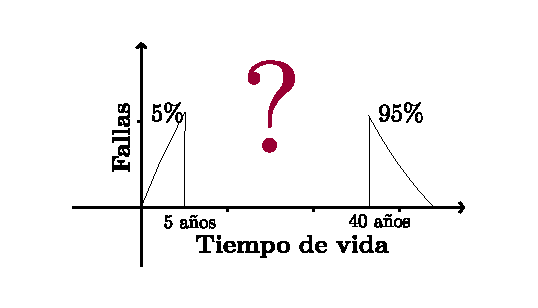
\includegraphics[scale=1]{apriori1.pdf}
\end{center}
\vspace{-1.5 cm}\caption{\bf Distribuci\'on predictiva a priori a modelar.}\label{dos}
\end{figure}

\noindent  Suponiendo que el $5\%$ de los transformadores fallan en los primeros 5 a\~nos (80 meses) y  que el $95\%$ de ellos ya fallaron a los $40$ a\~nos (480 meses) o antes, y 
si adem\'as $$T\sim \text{Weibull}(\eta^{*},\beta^{*})$$ 


\noindent es la variable aleatoria a priori que modela el tiempo de vida de los transformadores. La Figura \ref{dos} muestra la distribuci\'on a priori predictiva, con los cuantiles fijados en los extremos. Sin embargo el centro de la distribuci\'on debe ser modelada.\\[0.1cm]
\noindent La informaci\'on de los cuantiles se representa por:
$$P(T\leq 80)=0.05$$
y 
$$P(T\leq 480)=0.95.$$

\noindent Con esta informaci\'on es posible conocer  $\eta^{*}$ y  $\beta^{*}$  de la siguiente forma, se sabe que para una variable aleatoria Weibull
\begin{eqnarray*}
P(T\leq t) &=& 1-\exp\left\{-\left(\frac{t}{\eta}\right)^{\beta}\right\}
\end{eqnarray*}

Por lo tanto debemos resolver
\begin{eqnarray*}
0.05 &=& 1-\exp\left\{-\left(\frac{t}{\eta^{*}}\right)^{\beta^{*}}\right\}\\
0.95 &=& 1-\exp\left\{-\left(\frac{t}{\eta^{*}}\right)^{\beta^{*}}\right\}\\
\end{eqnarray*}

Resolviendo el sistema se llega a que

\begin{eqnarray*}
\beta^{*}&=& 1.955\\
\eta^{*}&=& 273.8
\end{eqnarray*}

\noindent Los par\'ametros encontrados describen el comportamiento a priori del tiempo de vida, no de los par\'ametros $\beta$  y $\eta$. Con ayuda de estos datos se pueden obtener los par\'ametros $a_1, b_1, a_2$ y $b_2$, que como lo mencionamos son los par\'ametros, para las distribuciones Gammas de  $\beta$ y $\eta$ respectivamente, notando lo siguiente:

\begin{enumerate}
\item[{\bf 1.-} ]
\noindent  Como $\beta^{*}= 1.955$, quiere decir que los valores que produzca la distribuci\'on Gamma con par\'ametros $a_1$ y $b_1$ oscilaran alrededor de estos valores. Similarmente como $\eta^{*}= 273.8$ significa que los valores que tome la distribuci\'on $Ga(a_2,b_2)$ estar\'an alrededor de 273.8 aproximadamente.
\item[{\bf 2.-} ]
\noindent De manera general  la funci\'on de densidad de una variable aleatoria Gamma con par\'ametros $a$ y $s$, representada como $Ga(a,s)$ es

$$f(x)=\frac{1}{s^a\Gamma(a)}x^{a-1}\exp\left\{\frac{x}{s}\right\}$$
y su valor esperado esta dado por:
\begin{eqnarray*}
E(X)&=& as.
\end{eqnarray*}

\noindent Del hecho de que  $\beta\sim $Gamma$(a_1,b_1)$ y  juntando las dos aseveraciones anteriores se tiene que: 
$\beta^{*}=1.955\approx E(\beta)=a_1b_1$, as\'i $$b_1=\frac{1.955}{a_1}.$$


De manera similar para  $\eta\sim $Gamma$(a_2,b_2)$ se obtiene

$\eta^{*}=273.8\approx E(\eta)=a_2b_2$, de donde
 $$b_2=\frac{273.8}{a_2}.$$

\end{enumerate}
Tanto $b_1$ como $b_2$ quedan expresadas en funci\'on de $a_1$ y $a_2$, que son los par\'ametros de forma para $\beta$ y $\eta$ respectivamente.\\[0.1cm]
Para  fijar $a_1$ y $a_2$, se  proponen distintos valores para estos par\'ametros. Para cada uno de los valores propuestos se obtienen sus respectivas $b_1$ y $b_2$, con lo que queda de manera expl\'icita establecidas las distribuciones a priori. Una vez teniendo estas a prioris se produce la distribuci\'on predictiva a priori y la funci\'on de riesgo. Luego se eval\'ua que tan cerca se encuentra la a priori predictiva de la informaci\'on que se esta modelando, para finalmente elegir $a_1$ y $a_2$ que ajusten  de manera razonable la informaci\'on a priori.

\noindent Realizando el procedimiento anterior se fijaron los siguiente valores
$a_1=25$,  $b_1 =0.092$, $a_2=12$ y  $b_2 =2.2$. La Figura \ref{risk1} muestra la densidad predictiva a priori  con los valores establecidos, y la Figura \ref{risk2} muestra la funci\'on de riesgo, se ha modelado de manera creciente. 

\begin{figure}
\centering
\includegraphics[scale=0.2]{app.pdf}
\vspace{-0.5cm}\caption{{\bf Funci\'on de densidad a priori.}\label{risk1}}
\end{figure}


\begin{figure}
\centering
\includegraphics[scale=0.2]{r2meses.pdf}
\vspace{-0.5cm}\caption{{\bf Funci\'on de riesgo a priori.}\label{risk2}}
\end{figure}

\section{Distribuci\'on  Posterior}
\noindent Recordando que  $T$ es la variable aleatoria que representa los tiempo de vida de los transformadores, su funci\'on de verosimilitud esta dada por (\ref{tiempos}) y las distribuciones (\ref{beta}), (\ref{eta}). 
La distribuci\'on posterior es 

\begin{eqnarray*}
f(\beta,\eta|T)&\propto&\mbox{Verosimilitud} \times \mbox{A priori} \\
&=& f(T|\beta,\eta)f(\beta,\eta)
\end{eqnarray*}
Suponiendo que existe independencia a priori, entre los par\'ametros $\beta$ y $\eta$ se tiene:

\begin{eqnarray}\label{pos}
f(\beta,\eta|T)&=&f(T|\beta,\eta)f(\beta,\eta)\\\nonumber
&=& f(T|\beta,\eta)f(\beta)f(\eta)\\\nonumber
&=& \prod_{e_i=0}\frac{\beta}{\eta}\left(\frac{t_i}{\eta}\right)^{\beta-1}\exp \left\{-\left(\frac{t_i}{\eta}\right)^{\beta}\right\}\prod_{e_i=1}\exp\left\{-\left(\frac{t_i}{\eta}\right)^{\beta}\right\}\\\nonumber
& &\frac{1}{b^a\Gamma(a)}\beta^{a-1}\exp\left\{-\frac{\beta}{b}\right\}\frac{1}{b_1^{a_1}\Gamma(a_1)}\eta^{a_1-1}\exp\left\{-\frac{\eta}{b_1}\right\}
\end{eqnarray}

\noindent La Ecuaci\'on (\ref{pos}) muestra que la distribuci\'on posterior de los par\'ametros, es una expresi\'on compleja y no f\'acil de evaluar.  En tales situaciones se recurre a la ayuda de m\'etodos computacionalmente intensivos que permiten simular una muestra de la distribuci\'on posterior, tales como algoritmos MCMC, que son ampliamente
utilizados en estas situaciones.

\begin{figure}[h]
\begin{minipage}[b]{0.5\linewidth}
 \includegraphics[scale=0.2]{pos1.pdf}
  \caption{{\small \bf Salida t-walk para $\beta.$}}
  \label{his1}
\end{minipage}
\begin{minipage}[b]{0.45\linewidth}
  \includegraphics[scale=0.2]{pos2.pdf}
  \caption{{\small \bf Salida t-walk para $\eta.$}}
  \label{his2}
\end{minipage}
\end{figure}

\noindent Para conocer la muestra de la distribuci\'on posterior se uso el lenguaje de programaci\'on R, y la funci\'on t-walk que permite obtener tal muestra [{\bf \ref{r}}]. Con la funci\'on t-walk se realizaron $900,000$ iteraciones para obtener la muestra deseada (\ref{pos}). Los resultados est\'an resumidos en las Figuras \ref{his1} y \ref{his2} que indican los valores en los que  se concentran $\beta$ y $\eta$. 
 
 \begin{figure}
\begin{center}
\includegraphics[scale=0.3]{logObj1.pdf} %logobj1
\end{center}
\vspace{-1cm} \caption{{\bf Dentro de t-Walk, se suele emplear, la funci\'on logaritmo de la distribuci\'on objetivo para evaluar la convergencia del m\'etodo. La gr\'afica muestra el comportamiento de esta funci\'on.}\label{mlog}}
\end{figure}

\begin{figure}
\begin{center}
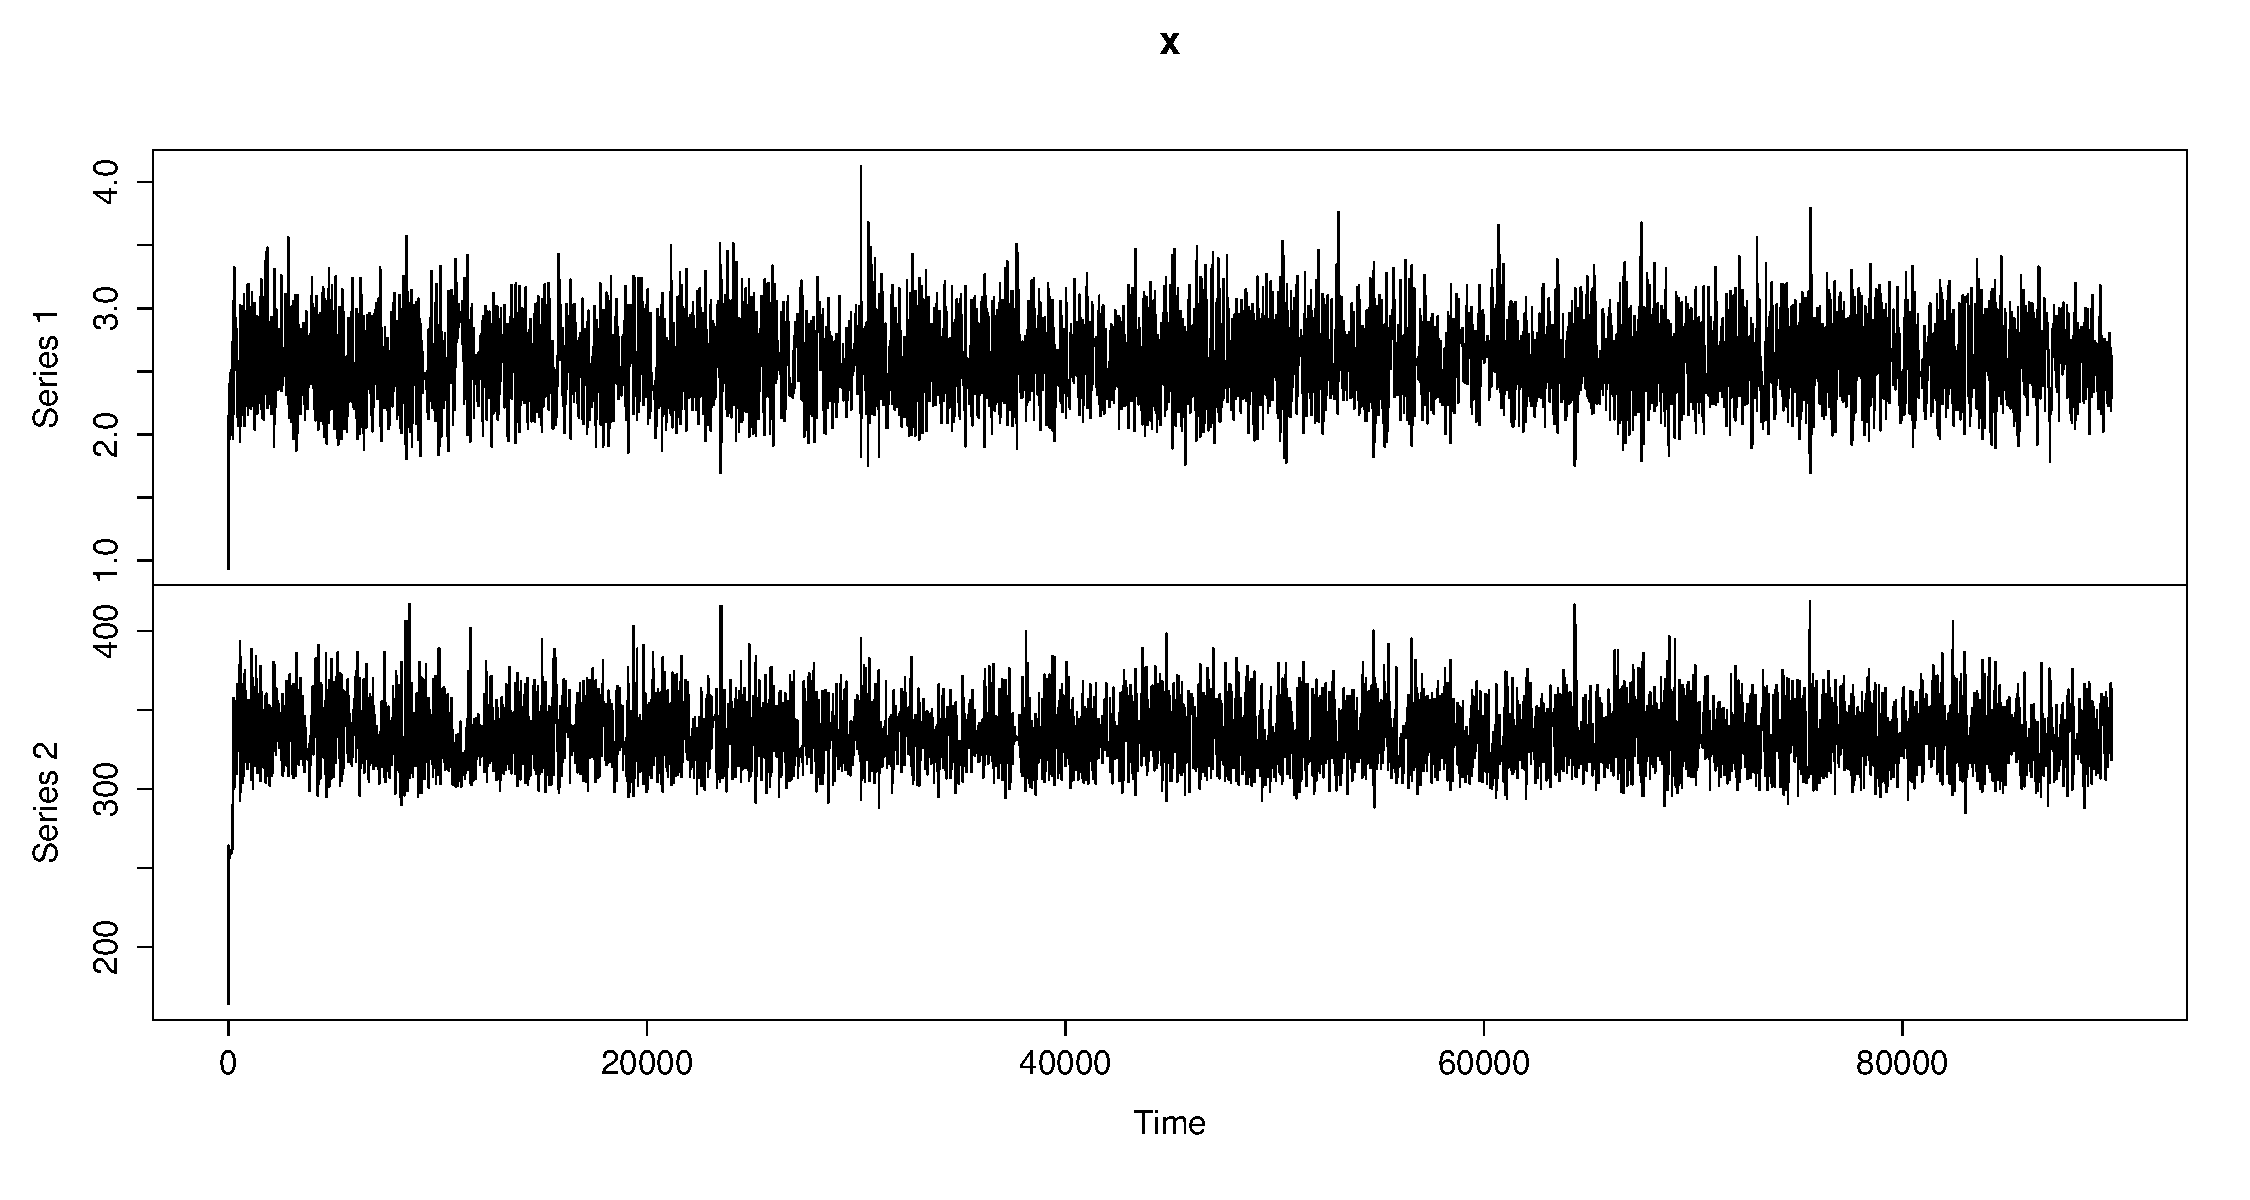
\includegraphics[scale=0.25]{serie.pdf}
\end{center}
\vspace{-1cm}\caption{{\bf Series de convergencia de los par\'ametros $\beta$ y $\eta$, proporcionados por la funci\'on t-Walk. La serie 1 corresponde a $\beta$ y la serie 2 a $\eta$.}\label{serie}}
\end{figure}

%\begin{figure}
%\begin{center}
%\includegraphics[scale=0.4]{corre1.pdf}
%\end{center}
%\vspace{-1cm}
%\caption{{\bf Muestra MCMC obtenida de la funci\'on t-Walk, graficada puntualmente con los valores de $\beta$ y $\eta$.}}
%\label{serie}
%\end{figure}

\noindent Las Figuras \ref{mlog} y \ref{serie}, muestran el an\'alisis de convergencia obtenido empleando la funci\'on t-walk. Observamos que la convergencia se da en un n\'umero de iteraciones relativamente peque\~no.\\[0.2cm]
\noindent Con la muestra se obtiene  la funci\'on de confiabilidad y la funci\'on de riesgo que se presentan en las Figuras \ref{CPos} y \ref{RPos} respectivamente. La confiabilidad decae lentamente. Se espera que a los 200 meses la probabilidad de que un transformador no falle es de 0.8. En la Tabla  \ref{conf} se muestran las probabilidades  de la funci\'on de confiabilidad, de los transformadores que segu\'ian operando despu\'es del 2006.

\begin{table}[h!]\small
\centering
\caption{\bf Confiabilidad de los transformadores que segu\'ian funcionando despu\'es del 2006.}\label{conf}
\vspace{.2cm}
\begin{tabular}{c|cccccc}
\toprule[0.6mm]
Meses de trabajo &8 &  20 & 32  & 56 & 80 &116  \\
\hline
Confiabilidad & 0.99 &0.99     &  0.99   &0.98 &0.97  &0.93 \\
\hline
Meses de trabajo &152 &164 &176& 188& 272& 296  \\
\hline
Confiabilidad & 0.87  &0.85   &  0.82     & 0.79 &0.55  &0.47 \\
\toprule[0.6mm]
\end{tabular}
\end{table}

\begin{figure}
\begin{center}
\includegraphics[scale=0.25]{ConPos.pdf}
\end{center}
\vspace{-0.5 cm} \caption{{\bf Confiabilidad posterior obtenida.}\label{CPos}}
\end{figure}



%\noindent Para evaluar el patr\'on de desgaste de la unidades en la Figura \ref{RPos} observamos la funci\'on de riesgo de los transformadores, esta crece de manera lenta.
\begin{figure}[h!]
\begin{center}
\includegraphics[scale=.25]{Rpos.pdf}
\end{center}
\vspace{-1 cm}{\caption{\bf  Tasa de falla mensual, empleando la muestra de la funci\'on t-Walk.}\label{RPos}}
\end{figure}
%\noindent Por lo tanto cabe recalcar que las gr\'aficas de las Figuras \ref{apripos}, \ref{CPos} y \ref{RPos} son aproximaciones empleando la muestra de la distribuci\'on posterior obtenida y aplicando (\ref{b}).

\newpage


\section{Almacenamiento de Transformadores}
\noindent Sea $n_0$ el n\'umero inicial de transformadores disponibles para reemplazar a los que fallan. Supongamos que al momento en que falla un transformador, se hace el pedido para sustituirlo y se espera un periodo de $\delta$ meses hasta que llega la orden. Mientras tanto este se reemplazar\'a por uno de los $n_0$ disponibles, si es que todav\'ia quedan en el almac\'en. Interesa determinar el valor de $n_0$, que asegure que a lo largo del periodo de tiempo analizado $(0,t)$, el almac\'en tenga los suficientes transformadores para cubrir las fallas a un costo m\'inimo.\\[0.2cm]
\noindent La Figura \ref{op} es un diagrama general de las etapas para  determinar la propuesta de inventario \'optima, empleando  la muestra de la distribuci\'on posterior y algunos costos que posteriormente estableceremos.

\begin{figure}[h!]
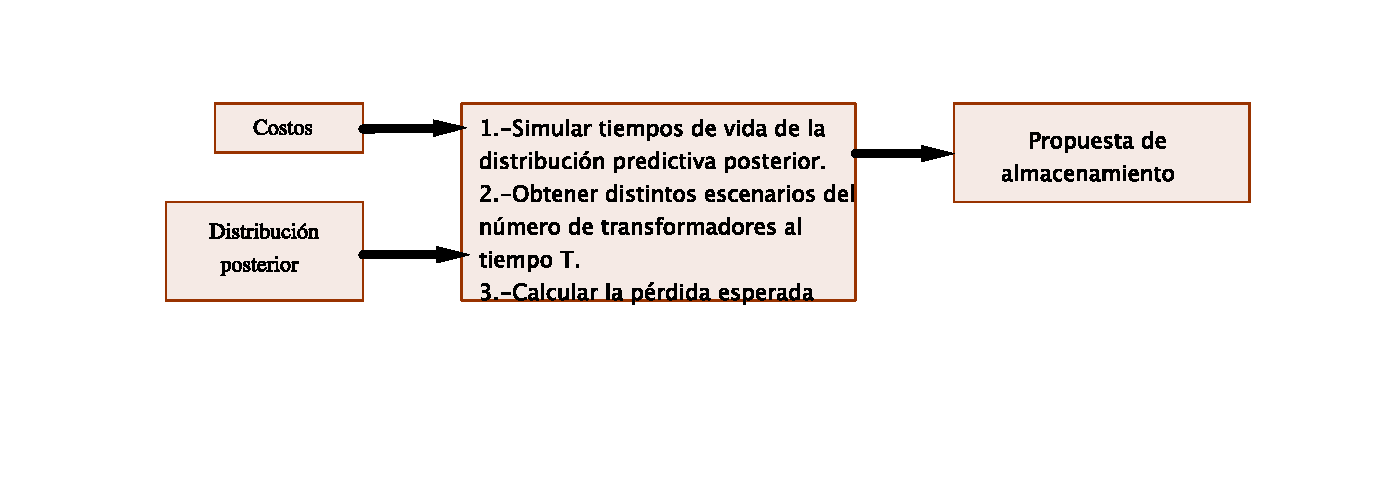
\includegraphics[scale=0.7]{final.pdf}
\vspace{-3cm}\caption{\bf Contrucci\'on del Plan de Almacenamiento.}\label{op}
\end{figure}


\noindent El procedimiento  para determinar el valor \'optimo de $n_0$, se basa en el c\'alculo de la funci\'on de p\'erdida esperada. Para esto simulamos tiempos de vida $t_1,t_2,\cdots, t_n$. El tiempo $t_i$, $i=1,\cdots,n$ provendr\'a de una distribuci\'on Weibull con par\'ametros $(\beta_i,\eta_i)$ de la muestra que ya se obtuvo de la distribuci\'on posterior. La Tabla \ref{ejee} contiene un conjunto de realizaciones $(\beta,\eta)$ de la distribuci\'on posterior y el $t_i$ correspondiente,

\begin{itemize}
\item $t_1=274$ es un dato que proviene de la distribuci\'on Weibull(2.228,347.37).
\item $t_2=542$ es un dato que proviene de la distribuci\'on Weibull(2.386,358.77).
\item $t_3=30.5$ es un dato que proviene de la distribuci\'on Weibull(3.534,350.55).
\item $\vdots$
\item $t_n=180$ es un dato que proviene de la distribuci\'on Weibull(2.456,340.51).
\end{itemize}
\noindent Los tiempos de vida simulados pueden ser considerados como una muestra, que resulta de una mezcla de distribuciones Weibull. Se puede demostrar que estos tiempos de vida provienen de la distribuci\'on posterior predictiva de $t$.
\begin{table}
\begin{center}

\vspace{-.3 cm}\caption{\bf Muestra MCMC.}\label{ejee}
\vspace{0.3cm}\begin{tabular}{cccc}
\toprule[0.6mm]
$i$&$\beta$ &$\eta$& $t_i$\\\toprule[0.6mm]
1&2.228 & 347.37 & 274
\\ 2&2.386 & 358.77 & 542
\\3&3.534 & 350.55 &305\\
 $\vdots$&$\vdots$ & $\vdots$ &$\vdots$
\\$n$& 2.456 & 340.51 & 180\\
\toprule[0.6mm]
\end{tabular}
\end{center}

\end{table}
\newpage

%\item {\bf Obtenci\'on de distintos escenarios del n\'umero de transformadores en el almac\'en}

\noindent Una vez establecidos los tiempos de falla de los transformadores. El n\'umero de transformadores en el almac\'en hasta el  tiempo $t$, depender\'a del n\'umero de fallas que ocurran durante el periodo de observaci\'on $(0,t)$, de $\delta$ y del n\'umero de transformadores que fijemos como iniciales $n_0$, es decir, es una funci\'on: $$n(t,n_0,\delta).$$
\noindent Para observar el comportamiento de $n(t,n_0,\delta)$ por simulaci\'on, se consideran tiempos de falla similares a los de la  Tabla \ref{ejee}. Se asume que al momento en que falla un transformador se solicita y llega $\delta$ meses despu\'es. Como solo se pide un transformador cuando alguno ha fallado, siempre tendremos en el almac\'en a lo m\'as $n_0$ transformadores.
\noindent De manera m\'as clara la forma de operar de $n(t,n_0,\delta)$, el n\'umero de transformadores disponibles en el almac\'en en el intervalo de tiempo de  $(0,t)$ es la siguiente: Al inicio del periodo $n(0,n_0,\delta)=n_0$, una vez que se llega a un tiempo de falla $t_1$ el valor de $n(t_1,n_0,\delta)$ ser\'a $n_0-1$ disminuye en uno y este se recuper\'a $\delta$ meses despu\'es. Si se llega a otro tiempo de falla antes de que llegue la orden entonces $n(\cdot)$ disminuir\'a en uno nuevamente, si ocurre lo contrario se recuperar\'a al menos en una unidad.\\

%\noindent Las gr\'aficas de algunas trayectorias simuladas de la funci\'on $n(t,n_0,\delta)$ para valores de $\delta=6,8$ y 12 meses  se muestran en las Figuras \ref{d6} \ref{d8} y \ref{d12}.

% \noindent Se decidi\'o analizar estos valores de $\delta$ , debido a que si los transformadores llegan en periodos menores de 6 meses, los valores de $n(t,n_0,\delta)$ no var\'ian de manera significativa. Por otro lado considerar periodos de espera m\'as largos que un a\~no parece ser un periodo grande de espera. 
\noindent Necesitamos establecer una funci\'on de p\'erdida, a partir de los escenarios simulados,  que permita saber la cantidad inicial adecuada de transformadores que deben tenerse en el almac\'en. 

%Rplot06
%\begin{figure}
%\begin{center}
%\includegraphics[scale=.3]{Rplot06.pdf}
%\end{center}
%\vspace{-1 cm} \caption{\bf Dos trayectorias obtenidas mediante simulaci\'on del n\'umero de transformadores en el almac\'en hasta el tiempo $t=200$ meses,  con $n_0=5$ transformadores al inicio del periodo de observaci\'on y $\delta=6$ meses de espera de llegada de los transformadores que se han pedido.}\label{d6}
%\end{figure}




\section{Funciones de P\'erdida}

\noindent Se proponen tres posibles pol\'iticas de inventario y posteriormente se describen sus funciones de p\'erdida. Se considera una pol\'itica de inventario, al planteamiento de una funci\'on de p\'erdida que refleje los costos de mayor inter\'es para la empresa.



\begin{description}
\item [Pol\'itica A] \hfill \\ 
La primera pol\'itica reflejar\'a el costo de quedarnos sin transformadores disponibles en el almac\'en. Estar\'a  enfocada a determinar el $n_0$ adecuado, tal que no permita que dentro del periodo de observaci\'on, el almac\'en se quede sin transformadores para cubrir todas sus demandas.
\item [Pol\'itica B] \hfill \\
La segunda pol\'itica adem\'as de considerar el costo de la pol\'itica A, adiciona el costo del lote inicial de transformadores en el almac\'en. 
\item [Pol\'itica C] \hfill \\
Esta \'ultima pol\'itica se centra en evaluar dos tipos de costos.
\begin{itemize}
\item[1.-] Costo de falta de transformadores por unidad de tiempo. Este costo tambi\'en considerado en las pol\'iticas anteriores.
\item[2.-] Costo de almacenamiento por cada unidad de tiempo.
\end{itemize}
\end{description}

\subsection{Pol\'itica A}

%\noindent Usando la Figura \ref{d6} es posible obtener la permanencia por debajo de cero de las trayectorias para distintos valores iniciales de $n_0$, lo cual se interpretar\'ia como el n\'umero de veces que la empresa se quedo sin transformadores para reemplazar. Es natural que entre m\'as peque\~no sea $n_0$, se permanece m\'as tiempo por debajo de cero y entre m\'as grande, la empresa se quedar\'a sin reservas por menos tiempo.\\[0.1cm]
\noindent Supongamos que se tiene una trayectoria como la de la Figura \ref{tr}, hasta un tiempo de $10$ meses y con $1$ transformador inicial de reserva. Supongamos adem\'as que al tiempo 3 falla un transformador, luego  $n(3)=0$. Despu\'es de un tiempo falla otro y no tenemos repuesto, entonces el n\'umero de transformadores en reserva es negativo ($n(4)=-1$). La p\'erdida asociada a partir de este tiempo, es el n\'umero de meses que permanece en esta situaci\'on (1 mes), multiplicada por un valor de $c$ unidades monetarias, que representa el costo de no poder cobrar la electricidad, por cada mes que no se tuvo un transformador de instrumento. Si se observa hasta $t=10$ entonces habr\'ia que sumar las p\'erdidas que representan el segundo bloque, que empieza en el tiempo $t=6$. Del bloque de $t=6$ a $t=7$ la p\'erdida involucra solamente a un transformador. Sin embargo en el intervalo de tiempo de $[7,9]$ meses la p\'erdida es m\'as grande, puesto que faltan dos transformadores para sustituir. La p\'erdida  ser\'a  los dos transformadores faltantes multiplicada por la longitud de tiempo que dure este hecho, (2 meses) por el valor de $c$. Por lo tanto la p\'erdida  total es:
\begin{eqnarray*}
c[1\cdot1 + 1\cdot1+2\cdot2+1\cdot1]
\end{eqnarray*} 
Lo que significa que la p\'erdida es la suma de las \'areas delimitadas por debajo de cero, multiplicada por $c$, donde $c$ se tiene que establecer con informaci\'on adicional. Sin perder generalidad se puede suponer $c=1$.\\[0.2cm]

\begin{figure}[h!]
\begin{center}
%\includegraphics[width=10cm,height=5cm]{Rplot01.png}
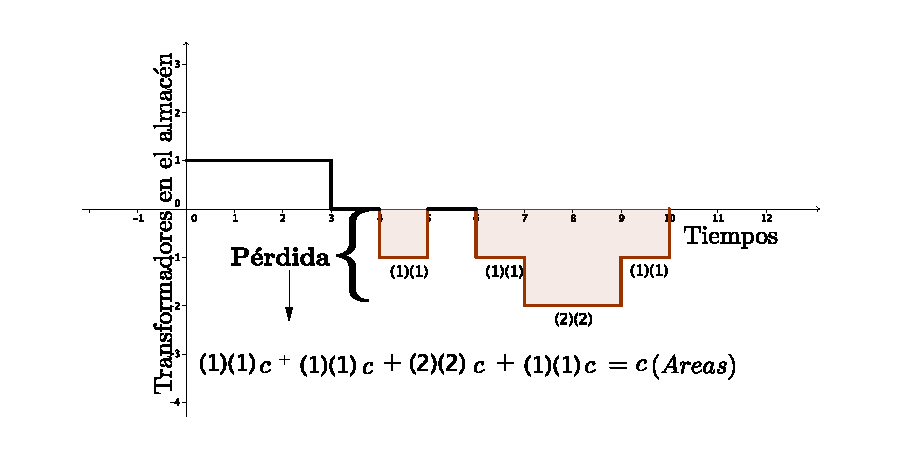
\includegraphics[scale=1]{tr1.pdf}
\end{center}
\vspace{-1.5 cm} \caption{\bf Almacenamiento de transformadores, hasta $10$ unidades de tiempo, mostrando la p\'erdida sobre ese per\'iodo.}\label{tr}
\end{figure}



\noindent De manera  general, podemos construir la funci\'on de p\'erdida asociada a la pol\'itica A, como se describe a continuaci\'on.\\[0.2cm]
\noindent Sean $\underline{T}=\{t_1,t_2,\cdots,t_n\}$ los tiempos de falla de los transformadores y 
$\underline{\ell}=\{\ell_1=t_1+\delta, \ell_2=t_2+\delta, \cdots, \ell_n=t_n+\delta\},$ los tiempos de llegada de los transformadores pedidos. 

\noindent  Definamos  $X(t;\underline{T})$ como el  n\'umero de transformadores en el almac\'en que se usaron para cubrir los tiempos de fallas hasta el tiempo $t$ y  $Y(t;\underline{T})$ el n\'umero de transformadores que se pidieron y llegaron antes del tiempo $t$. Luego $X(0)=n_0$ y $Y(0)=0$.\\[0.1cm]
\noindent Sea $Z(t,\underline{T})=X(t;\underline{T})+Y(t;\underline{T})$, indica el comportamiento de la funci\'on $n(t,n_0,\delta)$. Interesa conocer las veces en la cual esta permanece por debajo de cero.\\[0.1cm] 
\noindent La siguiente funci\'on restringue solo al \'area de inter\'es 
\[
W(t;\underline{T})=\left\{
\begin{array}{cl}
\displaystyle 0 & \mbox{ si } Z(t;\underline{T})\geq 0,\\                                                               Z(t)      &     \mbox{ si } Z(t;\underline{T})< 0  \\
\end{array}
\right.
\]

\noindent Una vez establecidas las funciones anteriores la funci\'on de p\'erdida esta dada por 

\begin{eqnarray}\label{LL}
L(t,\underline{T};\delta, n_0)=\int_{0}^{t} W(s;\underline{T}) ds,
\end{eqnarray}

\noindent dicho en palabras la p\'erdida esta representada por la integral sobre el periodo de observaci\'on, de las veces en las cuales el almac\'en se quedo sin transformadores disponibles para su uso.



\subsection{P\'erdida Esperada}

\noindent La funci\'on de p\'erdida dada por la Ecuaci\'on (\ref{LL}), depende de $n_0$, $\delta$ que son valores constantes y de \underline{T} que es una variable aleatoria, por lo tanto la funci\'on de p\'erdida es una funci\'on estoc\'astica, en el sentido de que depende de una variable aleatoria. Entonces la p\'erdida esperada tambi\'en es una funci\'on estoc\'astica, y esta dada por:
\begin{eqnarray}\label{ut}
U(t,n_0,\delta)=E(L(t,\underline{T},n_0, \delta)).
\end{eqnarray}

\noindent Por la ley de los grandes n\'umeros, la manera de estimar la Ecuaci\'on (\ref{ut}), es mediante la  expresi\'on:

\begin{eqnarray}\label{utqq}
\hat{U}(t,n_0,\delta)=\frac{1}{M} \sum_{s=1}^{M}\int_{0}^{t} W(y,\underline{T}_s) dy,
\end{eqnarray}
 donde $M$ es el n\'umero de $\underline{T}_s$ simulados.
\noindent Para calcular la expresi\'on (\ref{utqq}) por simulaci\'on se hace de la siguiente manera:

\begin{enumerate}
\item Se simulan $M$ trayectorias de tiempos de vida, dicho en otras palabras $M$ vectores del tipo $\underline{T}$.
\item Para cada trayectoria se calcula la Ecuaci\'on (\ref{LL}).
%que indica la p\'erdida en toda la trayectoria de tiempos simulada.
\item De los $M$ valores obtenidos,  se obtiene el promedio de ellos, que ser\'a la p\'erdida esperada.
%\item Una vez que se tienen las $M$, trayectorias y sus sumas asociadas, se calcula el promedio de las sumas, los cuales representan la p\'erdida esperada (Ecuaci\'on \ref{utqq}).\\[0.2cm]
\end{enumerate}

\noindent De acuerdo a los pasos anteriores, se realizaron 1000 simulaciones para cada pareja $$(\delta_i,n_{0_j})$$ donde $\delta_i=6, 8$ y 12 meses, $n_{0_j}=1,2,\cdots, 24$ que representa el n\'umero de transformadores al inicio del periodo. Luego se obtuvo el promedio de las funciones de p\'erdida, calculadas en cada una de las 1000 simulaciones para cada pareja, se consider\'o un tiempo de observaci\'on de 40 a\~nos (480 meses).\\[0.1cm]

\noindent La Figura \ref{d6s} muestra la gr\'afica de las p\'erdidas esperadas para $\delta=6,8,12$ meses.  Observamos que para valores de $n_0$ peque\~nos, 
las perdidas esperadas son grandes. A medida que $n_0$ crece, los promedios disminuyen. Al considerarse tiempos de espera m\'as largos, los costos tambi\'en se incrementan, las mayores p\'erdidas se tienen cuando $\delta=12$, para este periodo de espera se necesitan al menos 24 transformadores al inicio del periodo de observaci\'on (Tabla \ref{c777}). Para $\delta=8$ se requieren 15 transformadores (Tabla  \ref{c33333} )y para $\delta=6$ se necesitan 15 transformadores en el almac\'en (Tabla \ref{c1}).



\begin{figure}[h!]
\begin{center}
\includegraphics[scale=0.35]{poA.pdf}
\end{center}
\vspace{-1 cm} \caption{\bf P\'erdidas Esperadas con la Pol\'itica A, usando $t=480$, $\delta=6,8,12$ y Differentes Valores de $n_0$.}\label{d6s}
\end{figure}




\begin{table}[h!]\small
\centering
\caption{\bf Pol\'itica A: Valores de las P\'erdidas Esperadas con $\delta=6$.}\label{c1}
\vspace{0.3 cm}\begin{tabular}{ccccccccc}
\toprule[0.6mm]

$\bf{n_0}$&\bf{1} &                   \bf{2} &                   \bf{3} &                   \bf{ 4 }&                    \bf{ 5}&              \bf{ 6} &               \bf{ 7} & \bf{8} \\
\hline
$\mbox{\bf Promedio}$&1029.433  &697.822&  437.725&  251.263 & 131.085 &  62.514 &  27.148 &  11.136 \\	
\hline
$\bf{n_0}$&\bf{9} &                \bf{ 10}&              \bf{      11} &                   \bf{ 12} &               \bf{      13}&              \bf{14} &  \bf{ 15} & \bf{16 }   \\
\hline
$\mbox{\bf Promedio}$&	 4.003  &  1.343 &   0.446 &   0.167&    0.028 &   0.040 &   0.000&    0.000\\ 
	 \hline
	
$\bf{n_0}$&\bf{17} &     \bf{ 18}&   \bf{19}&   \bf{ 20} &           \bf{   21}&                \bf{  22}  & \bf{23} & \bf{24}  \\
\hline
$\mbox{\bf Promedio}$&  0.000 &   0.000&    0.000 &   0.000   & 0.000  &  0.000 &   0.000 & 0.000\\
\toprule[0.6mm]
\end{tabular}

\end{table}


\begin{table}[h!]\small
\centering
\caption{\bf Pol\'itica A: Valores de las P\'erdidas Esperadas con $\delta=8$.}\label{c33333}
\vspace{0.3 cm}\begin{tabular}{ccccccccc}
\toprule[0.6mm]
$\bf{n_0}$&\bf{1} &                   \bf{2} &                   \bf{3} &                   \bf{ 4 }&                    \bf{ 5}&              \bf{ 6} &               \bf{ 7} & \bf{8} \\
\hline
$\mbox{\bf Promedio}$&1483.721 &1118.711  &799.610  &539.082 & 338.785  &200.591  &109.192  & 55.774 \\
\hline
$\bf{n_0}$&\bf{9} &                \bf{ 10}&              \bf{      11} &                   \bf{ 12} &               \bf{      13}&              \bf{14} &  \bf{ 15} & \bf{16 }   \\
\hline
$\mbox{\bf Promedio}$&	   25.935  & 11.184  &  4.376  &  1.637   & 0.733   & 0.219   & 0.081  &  0.032  \\
	 \hline
	
$\bf{n_0}$&\bf{17} &     \bf{ 18}&   \bf{19}&   \bf{ 20} &           \bf{   21}&                \bf{  22}  & \bf{23} & \bf{24}  \\
\hline
$\mbox{\bf Promedio}$&   0.004 &   0.003&    0.000 &   0.000   & 0.000  &  0.000 &   0.000 & 0.00\\
\toprule[0.6mm]
\end{tabular}

\end{table}


\begin{table}[h!]\small
\centering
\caption{\bf Pol\'itica A: Valores de las P\'erdidas Esperadas con $\delta=12$.}\label{c777}
\vspace{.3cm}\begin{tabular}{ccccccccc}
\toprule[0.6mm]
$\bf{n_0}$ &\bf{1} &                   \bf{2} &                   \bf{3} &                   \bf{ 4 }&                    \bf{ 5}&              \bf{ 6} &               \bf{ 7} & \bf{8} \\
\hline
{\bf Promedio} & 2411.0  & 2008.7 &1640.9 &1305.0&1002.0 & 740.5 & 526.5 & 357.3    \\
\hline
$\bf{n_0}$&\bf{9} &                \bf{ 10}&              \bf{      11} &                   \bf{ 12} &               \bf{      13}&              \bf{14} &  \bf{ 15} & \bf{16 }   \\
\hline
{\bf Promedio}&	 222.7 & 137.1 &  78.0 &   41.8 &  21.1  &   9.8  &    4.8  &  2.3    \\
	 \hline
	
$\bf{n_0}$&\bf{17} &     \bf{ 18}&   \bf{19}&   \bf{ 20} &           \bf{   21}&                \bf{  22}  & \bf{23} &\bf {24}  \\
\hline
   {\bf Promedio} &  0.9    &  0.34 &   0.09 &   0.03 &   0.01 &   0.02 &   0.003  & 0.00\\
\toprule[0.6mm]
\end{tabular}

\end{table}
%------------------------------------------------------------------------------------------------------------------------------------------------------------
\newpage
\noindent Cabe destacar que los valores considerandos de $\delta$'s y $t=480$ meses, se utilizaron para  ilustrar la metodolog\'ia sugerida, puesto que no se tiene acceso a los valores reales. Sin embargo con la metodolog\'ia propuesta, cualesquiera que fueran los valores reales, los c\'alculos anteriores pueden realizarse.



\subsection{Pol\'itica B}
\noindent Dentro de esta secci\'on se emplea la pol\'itica B, para establecer la funci\'on de p\'erdida utilizando los siguientes costos:

\begin{description}

\item [Costo 1:] \hfill \\El costo de no poder cobrar la electricidad durante un  periodo de tiempo donde no hab\'ia transformadores en reserva, considerado en la secci\'on anterior.
\item [Costo 2:] \hfill\\El costo de almacenamiento por unidad e de tiempo.
\end{description}

\noindent Sea $C$ el costo de no poder cobrar la electricidad en una unidad de tiempo. Luego el costo de almacenar un transformador por una unidad de tiempo, lo podemos expresar en t\'erminos de $C$ como
 $rC$. Asumiendo que el {\bf Costo 1} es mayor que el {\bf Costo 2} entonces $r \in(0,1)$.\\[0.1cm]
 
 
 
\noindent  La funci\'on de p\'erdida considerando el {\bf costo 1} y el costo inicial de almacenamiento durante la primera unidad de tiempo es:
\begin{eqnarray*}
L(t,\underline{T},\delta, n_0)=C\int_{0}^{t} W(s;\underline{T})  ds + rn_0C \mbox{ },
\end{eqnarray*}

\noindent Suponiendo $C=1$, es decir, una unidad de dinero. La p\'erdida  se simplifica a: 
\begin{eqnarray}\label{LL1}
L(t,\underline{T},\delta, n_0)=\int_{0}^{t} W(s;\underline{T})  ds + rn_0,
\end{eqnarray}
La p\'erdida esperada puede calcularse como:
\begin{eqnarray*}
\hat{U}(t,n_0,\delta)=\frac{1}{M} \sum_{s=1}^{M}\left(\int_{0}^{t} W(y;\underline{T}_s) dy + n_0r\right)
\end{eqnarray*}


 \noindent donde $M$ es el n\'umero de $\underline{T}$'s simulados. Es decir, a la p\'erdida  planteada en la secci\'on anterior se le suma la recta $rn_0$, como funci\'on de $n_0$. Esta recta representa los costos de almacenamiento de los transformadores inciales.
%Hemos entonces construido una nueva funci\'on de p\'erdida que considere las dos p\'erdidas, de tener almacenados transformadores extras y el costo de quedarnos sin ellos.\\[0.2cm]

\noindent Asignando valores a $r$, se puede observar la manera de comportarse de esta funci\'on de p\'erdida  (\ref{LL1}) y los valores de $n_0$'s que esta funci\'on proporcione. La manera de estimar la p\'erdida esperada es por medio de simulaciones (como se describe en la pol\'itica A). 
A continuaci\'on se muestran los resultados.\\[.2cm]
\noindent En la Figura \ref{u01p6} observamos las p\'erdidas esperadas suponiendo distintos n\'umeros de transformadores iniciales, y $r=0.1$, la recta mostrada corresponde a $n_0r$. A partir de cierto punto la p\'erdida esperada esta sobre la misma linea que la recta, esto indica que a partir del primer punto en el cual se da este parecido, la p\'erdida esperada se ve afectada por los costo de almacenamiento. 


\noindent En la Tabla \ref{r11} mostramos los valores graficados de la Figura \ref{u01p6}. De $n_0=1$ hasta 13, la p\'erdida esperada decrece, a partir de $n_0=13$ la p\'erdida empieza a crecer lentamente. Por lo que el $n_0$ \'optimo para $\delta=6$ meses y $r=0.1$ es 13 transformadores. Un comportamiento similar se observa en el resto de las Figuras mostradas (\ref{fi} y \ref{r0.5delta6}.
%%%%%%%%%%%%%%%%%#########################
%Delta=6

\begin{figure}[h!]
\begin{center}
\includegraphics[scale=0.3]{utilpeso01delta61.pdf}
\end{center}
\vspace{-1 cm}\caption{\bf P\'erdidas Esperadas con la Pol\'itica B, usando $\delta=6$ y r=0.1}\label{u01p6}
\end{figure}

\begin{table}[h!]\small
\centering
\caption{\bf Pol\'itica B: Valores de las P\'erdida  Esperadas con $\delta=6$, $r=0.1$.}\label{r11}
\begin{tabular}{ccccccccc}
\toprule[0.6mm]
$\bf{n_0}$ &\bf{1} &                   \bf{2} &                   \bf{3} &                   \bf{ 4 }&                    \bf{ 5}&              \bf{ 6} &               \bf{ 7} & \bf{8} \\
\hline
${\bf Promedio}$ &  
 1026.86 &  701.26 & 441.20 & 248.58 & 132.61  & 61.29 &  27.04&   12.30 \\
\hline
$\bf{n_0}$& \bf{9} &                \bf{ 10}&              \bf{      11} &                   \bf{ 12} &               \bf{      13}&              \bf{14} &  \bf{ 15} & \bf{16 }   \\
\hline
${\bf Promedio}$&	  5.50 &   2.71 &   1.50 &   1.39 &   1.34 &   1.43  &  1.50 &   1.60    \\
	 \hline
	
$\bf{n_0}$&\bf{17} &     \bf{ 18}&   \bf{19}&   \bf{ 20} &           \bf{   21}&                \bf{  22}  & \bf{23} & \bf{23}  \\
\hline
${\bf Promedio}$&    1.70  &1.80 &   1.90 &   2.00  &  2.10  &  2.20 &   2.30  &   2.40 \\
\toprule[0.6mm]
\end{tabular}

\end{table}





 
%%%%%%%%%%%%%%%%%%%%%%%%%%%%%%%%%%%

\noindent Para un periodo de reemplazo $\delta$=8 meses, los resultados de la p\'erdida  esperada se ven en la Figura \ref{fi} y los valores graficados en la Tabla \ref{r12}. A partir de $n_0=14$ la p\'erdida  esperada empieza a crecer.
%delta8
%t=480 siempre!!!!!!!!!!!!!
\begin{figure}[h!]
\begin{center}
\includegraphics[scale=0.3]{utilpeso01delta8.pdf}
\end{center}

\vspace{-1 cm}\caption{\bf P\'erdidas Esperadas con la Pol\'itica B, usando $\delta=8$ y r=0.1}\label{fi}
\end{figure}
\begin{table}[h!]\small
\centering
\caption{\bf Pol\'itica B: Valores de las P\'erdidas Esperadas con $\delta=8$, $r=0.1$.}\label{r12}
\begin{tabular}{ccccccccc}
\toprule[0.6mm]
$\bf{n_0}$ &\bf{1} &                   \bf{2} &                   \bf{3} &                   \bf{ 4 }&                    \bf{ 5}&              \bf{ 6} &               \bf{ 7} & \bf{8} \\
\hline
${\bf Promedio}$ & 1485.90 &1127.06 & 798.25  &545.79 & 347.76 & 205.38 & 114.38 &  56.49  \\
\hline
$\bf{n_0}$&\bf{9} &                \bf{ 10}&              \bf{      11} &                   \bf{ 12} &               \bf{      13}&              \bf{14} &  \bf{ 15} & \bf{16 }   \\
\hline
${\bf Promedio}$&	27.63 &  12.22 &   6.74 &   3.51  &  2.11&    1.49 &   1.52 &   1.61 \\
	 \hline
	
$\bf{n_0}$&\bf{17} &     \bf{ 18}&   \bf{19}&   \bf{ 20} &           \bf{   21}&                \bf{  22}  & \bf{23} &\bf{24}  \\
\hline
${\bf Promedio}$ &  1.72 &  1.80  &  1.90 &   2.00   & 2.10   & 2.20 &   2.30 &  2.40  \\
\toprule[0.6mm]
\end{tabular}

\end{table}


%
%%%%%%%%%%%%%%%%%%%%%%%%%%%%
\newpage
\noindent En la Figura \ref{r0.5delta6} se muestra la grafica de la p\'erdida esperada con $r=0.5$. De la Tabla \ref{tt7} se deduce que  el n\'umero de transformadores iniciales, adecuados en el almac\'en es $n_0=11$.
%delta6 peso=0.5
\begin{figure}[h!]
\begin{center}
\includegraphics[scale=0.3]{utipeso05delta6.pdf}
\end{center}
\vspace{-1 cm} \caption{\bf P\'erdidas Esperadas con la Pol\'itica B, usando $\delta=6$ y r=0.5}\label{r0.5delta6}
\end{figure}


\begin{table}\small
\centering
\caption{\bf Pol\'itica B. Valores de las P\'erdidas Esperadas con $\delta=6$, $r=0.5$.}\label{tt7}
\begin{tabular}{ccccccccc}
\toprule[0.6mm]
$\bf{n_0}$ &\bf{1} &                   \bf{2} &                   \bf{3} &                   \bf{ 4 }&                    \bf{ 5}&              \bf{ 6} &               \bf{ 7} & \bf{8} \\
\hline
{\bf Promedio} & 1030.57 & 699.97&  432.87 & 249.35 & 135.35  & 65.35 &  31.56 &  14.56  \\
\hline
$\bf{n_0}$&\bf{9} &                \bf{ 10}&              \bf{      11} &                   \bf{ 12} &               \bf{      13}&              \bf{14} &  \bf{ 15} & \bf{16 }   \\
\hline
{\bf Promedio}&	9.15 &   6.56 &   5.65  &  6.08  &  6.57 &   7.00  &  7.50 & 8.00  \\
	 \hline
	
$\bf{n_0}$&\bf{17} &     \bf{ 18}&   \bf{19}&   \bf{ 20} &           \bf{   21}&                \bf{  22}  & \bf{23} &  \bf{24}\\
\hline
{\bf Promedio} &    8.50 &   9.00  &  9.50  &  10.0 &  10.50 &  11.00  & 11.50& 12.00\\
\toprule[0.6mm]
\end{tabular}

\end{table}

 \subsection{Pol\'itica C}
\noindent Esta \'ultima pol\'itica considera los dos costos empleados en la Pol\'itica B por unidad de tiempo. La funci\'on de p\'erdida, esta dada por la siguiente expresi\'on.


\begin{eqnarray}
L(t,\underline{T},\delta,n_0)=\int_{0}^{t} W(s,\underline{T}) ds + r \int_{0}^{t} A(s,\underline{T}) ds
\end{eqnarray}
donde:
\[
A(t,\underline{T})=\left\{
\begin{array}{cl}
\displaystyle 0 & \mbox{ si } Z(t,\underline{T})\leq 0,\\                                                               Z(t)      &     \mbox{ si } Z(t,\underline{T})>0  \\
\end{array}
\right.
\]

\noindent La funci\'on $A(t,\underline{T})$ refleja las p\'erdidas que existen por almacenar transformadores. Para este caso la p\'erdida esperada se calcula como:
\begin{eqnarray}\label{LL3}
\hat{U}(t,n_0,\delta)&=& \frac{1}{M}\sum_{s=1}^M \left(     \int_{0}^{t} W(s,\underline{T}) ds + r \int_{0}^{t} A(s,\underline{T}) ds       \right).
\end{eqnarray}

\noindent Para evaluar la Ecuaci\'on (\ref{LL3}) procedemos de la misma manera que en las pol\'iticas anteriores.  A continuaci\'on se mostraran algunas gr\'aficas (Figuras \ref{u38i} y \ref{u36i}) y Tablas  (\ref{u38t} y \ref{u36t}) de los resultados.

\begin{figure}[h!]
\begin{center}
\includegraphics[scale=0.3]{uA8.pdf}
\end{center}
\vspace{-1 cm} \caption{\bf P\'erdidas Esperadas con la Pol\'itica C, usando $\delta=6$ y $r=0.01$}\label{u38i}
\end{figure}


\begin{table}[h!]\small
\centering
\caption{\bf Pol\'itica C. Valores de las P\'erdidas Esperadas con $\delta=6$ y $r=0.01$.}\label{u38t}
\begin{tabular}{ccccccccc}
\toprule[0.6mm]
$\bf{n_0}$&\bf{1} &                   \bf{2} &                   \bf{3} &                   \bf{ 4 }&                    \bf{ 5}&              \bf{ 6} &               \bf{ 7} & \bf{8} \\
\hline
{\bf Promedio}& 611687.9 &413680.9 &256825.8& 150424.5&  75977.0  &37610.2 & 16419.3 &   6576.2  \\
\hline
$\bf{n_0}$&\bf{9} &                \bf{ 10}&              \bf{      11} &                   \bf{ 12} &               \bf{      13}&              \bf{14} &  \bf{ 15} & \bf{16 }   \\
\hline
{\bf Promedio}&	    2408.7  & 1021.0 &   190.9 &   140.7 & 138.1  &  117.3  &  114.6 &   124.0  \\
	 \hline
	
$\bf{n_0}$&\bf{17} &     \bf{ 18}&   \bf{19}&   \bf{ 20} &           \bf{   21}&                \bf{  22}  & \bf{23} &  \bf{24}\\
\hline
{\bf Promedio}&  133.4 &   144.0 &152.2    &163.5 &   172.2  &  180.6 &   190.4 &199.2\\
\toprule[0.6mm]
\end{tabular}

\end{table}
%#---------------------------------------------------------------------------------------------------------------------------------------------------------%r=0.1
\begin{figure}[h!]
\begin{center}
\includegraphics[scale=0.3]{uA6puntouno.pdf}
\end{center}
\vspace{-1 cm} \caption{\bf P\'erdidas Esperadas con la Pol\'itica C, usando $\delta=6$ y $r=0.1$.}\label{u36i}
\end{figure}


\begin{table}[h!]\small
\centering
\caption{\bf Pol\'itica C: Valores de la P\'erdidas Esperadas con $\delta=6$ y $r=0.1$.}\label{u36t}
\begin{tabular}{ccccccccc}
\toprule[0.6mm]
$\bf{n_0}$&\bf{1} &                   \bf{2} &                   \bf{3} &                   \bf{ 4 }&                    \bf{ 5}&              \bf{ 6} &               \bf{ 7} & \bf{8} \\
\hline
{\bf Promedio}& 606757 & 417457 &258881& 151181 & 78446 & 38066 & 15675&  6799  \\
\hline
$\bf{n_0}$&\bf{9} &                \bf{ 10}&              \bf{      11} &                   \bf{ 12} &               \bf{      13}&              \bf{14} &  \bf{ 15} & \bf{16 }   \\
\hline
{\bf Promedio}&	    2385 &  1332&   563 &   526 &   566 &   576&  628  &  686   \\
	 \hline
	
$\bf{n_0}$&\bf{17} &     \bf{ 18}&   \bf{19}&   \bf{ 20} &           \bf{   21}&                \bf{  22}  & \bf{23} &  \bf{24}\\
\hline
{\bf Promedio}&   732  &  785 &  836&   889  &  941&  992 &  1046 &  1098\\
 \toprule[0.6mm]
\end{tabular}

\end{table}


\begin{figure}[h!]
\begin{center}
\includegraphics[scale=0.3]{puntocinco.pdf}
\end{center}
\vspace{-1 cm}\caption{\bf P\'erdidas Esperadas con la Pol\'itica C, usando $\delta=8$, $r=0.5$.}\label{u385i}
\end{figure}

\noindent Las gr\'aficas presentadas tienen un comportamiento similar, a las que previamente ya hab\'iamos obtenido. La tendencia es bajar para los primeros valores de $n_0$ y posteriormente subir. La diferencia m\'as significativa radica en  el hecho de que los costos, a los cuales se minimiza $n_0$ son mucho mayores que en las anteriores funciones de p\'erdida. Este hecho se debe a que dentro de esta \'ultima pol\'itica se consideran costos de almacenamiento por cada unidad de tiempo.

\section{Conclusiones}
\noindent A lo largo de este cap\'itulo se han obtenido valores  para el n\'umero de transformadores iniciales que se deben de tener en el inventario. La Tablas  \ref{taba1},\ref{resu2} y \ref{resuFF},  resumen los valores obtenidos y mencionados en las secciones anteriores.
\begin{table}[h!]\small
\begin{center}
\caption{\bf Resultados de la Pol\'itica A.}\label{taba1}
\vspace{0.3cm}\begin{tabular}{ccc}
\toprule[0.6mm]
  $\delta$ & $n_0$ & costo\\
\toprule[0.6mm]
  6 & 15 &0.00\\
  8&19& 0.00\\
  12&24 & 0.00\\
\toprule[0.6mm]
\end{tabular}
\end{center}
%\caption{$n_0$'s \'optimos considerando solo el costo de quedarnos sin transformadores.}\label{resu1}
\end{table}


\noindent En la Tabla \ref{taba1} se muestran los valores \'optimos de transformadores iniciales que deben tenerse en el almac\'en, para un periodo de tiempo de $40$ a\~nos con diferentes valores de $\delta$, bajo la pol\'itica A. Es normal observar que entre mayor sea el periodo de espera de un transformador solicitado, mayor ser\'a el n\'umero de transformadores requeridos para el almacenamiento. Los costos asociados son cero, indica que a partir de la cantidad $n_0$ de transformadores, no habr\'a p\'erdidas en cuanto a la falta de ellos. Las conclusiones anteriores corresponden solo al considerarse un costo. Para ambos costos, los resultados se muestran en la Tabla \ref{resu2}, para diferentes valores de $r$ y usando la pol\'itica B.


\begin{table}[ht]\small
\begin{center}
\caption{\bf Resultados de la Pol\'itica B.}\label{resu2}
\vspace{0.3cm}\begin{tabular}{cccc}
\toprule[0.6mm]
 $\delta$ & $n_0$  & costo& $r$\\
\toprule[0.6mm]
  6   & 14 & 0.14& 0.01\\
  8   & 17 & 0.16& 0.01\\
  12 & 22  & 0.20 & 0.01\\
  \hline
  6   & 13 & 1.34& 0.1\\
  8   & 14 & 1.49& 0.1\\
  12 & 20 & 2.00& 0.1\\
  \hline
  6   & 11& 5.65 &0.5 \\
  8   & 14 &7.11 & 0.5 \\
  12 & 18 &9.16 &0.5\\
\toprule[0.6mm]
\end{tabular}
\end{center}

\end{table}






\noindent De la Tabla  \ref{resu2} notamos que al a\~nadir costos de almacenamiento inicial, los costos para $n_0$ obtenidos no se minimizan a cero.\\[0.1cm]
\noindent Cuando $r=0.01$, indica que si el costo de no tener un transformador disponible es $c$, entonces el costo por tener un transformador almacenado y no usarlo es $rc=\displaystyle\frac{1}{100}c$. El quedarse sin un transformador es 100 veces m\'as caro que almacenar un transformador y no usarlo. Para un periodo de espera $\delta=8$ meses se obtiene que  $n_0=17$ y el costo asociado es $0.16$. El valor de $n_0$ es menor que el obtenido en la Tabla \ref{taba1}, pero el costo es mayor. Esto se debe a que la funci\'on de p\'erdida dada por la Ecuaci\'on (\ref{LL1}), involucra costos de almacenamiento, entonces la p\'erdida esperada buscar\'a tener la m\'inima cantidad de transformadores al costo m\'as peque\~no posible. Los resultados obtenidos para $r=0.01$ no son tan significativamente variante de los mostrados en la Tabla \ref{taba1}, ya que la proporci\'on $r$, es peque\~na. Las diferencias notorias son para valores de $r$ mayores.\\[0.1cm]

\noindent Al tener $r=0.1$, indica que el quedarnos sin transformadores en 10 veces m\'as costoso que tener almacenados transformadores. Los costos a los cuales se minimiza la p\'erdida esperada oscilan de $1$ a $2$ unidades de $c$ y los valores de $n_0$ son menores o iguales al considerar solo la pol\'itica A. Un efecto similar ocurre al considerar $r=0.5$. \\[0.1cm]
 A medida que $r$ crece, el valor de $n_0$ se hace peque\~no y el costo aumenta. Entre mayor sea el costo de almacenamiento, se buscar\'a tener menos transformadores.\\[0.2cm]
Finalmente para la pol\'itica C, los costos aumentan significativamente respecto a la pol\'itica A y B. Ahora se consideran costos por unidad de tiempo, tanto de falta de ellos como de almacenamiento. As\'i que se busca no  tener transformadores en el almac\'en pero tampoco necesitarlos, raz\'on por la cual, los costos   de optimizaci\'on para esta pol\'itica son altos y los valores de $n_0$ asociados son menores a los de las pol\'iticas anteriores.
\begin{table}[h!]\small
\begin{center}
\caption{\bf Resultados de la Pol\'itica C.}\label{resuFF}
\vspace{0.3cm}\begin{tabular}{cccc}
\toprule[0.6mm]
 $\delta$ & $n_0$  & costo& $r$\\
\toprule[0.6mm]
  6   & 15 & 114& 0.01\\
  8   & 16 & 119& 0.01\\
  12 & 20  & 145 & 0.01\\
  \hline
  6   & 12 & 526& 0.1\\
  8   & 15 & 606& 0.1\\
  12 & 20 & 779& 0.1\\
  \hline
  6   & 11& 2209&0.5 \\
  8   & 14&2524 & 0.5 \\
  12 & 15 &8836 &0.5\\
\toprule[0.6mm]
\end{tabular}
\end{center}

\end{table}


\noindent Una vez presentadas las funciones  de p\'erdida planteadas y los resultados obtenidos. La pregunta de mayor inter\'es es ?`C\'ual es la m\'as adecuada?. La aplicaci\'on de cualquiera de ellas depender\'a de las condiciones reales del problema, determinadas por la empresa. Por ejemplo, si dentro la empresa, el principal costo a minimizar es el de no poder cobrar la electricidad, en el tiempo que no se tenga un transformador de reemplazo, entonces aplicar\'iamos la propuesta A. Si  por otra parte la empresa determina que adem\'as de considerar el costo de no tener transformadores disponibles, le  interesa minimizar el costo de almacenamiento $n_0$, al inicio de su periodo de observaci\'on, m\'as el costo de no tenerlos. Y justifica que a lo largo del tiempo el adquirir solo un transformador  a la vez no le afecta de manera significa, pero que el adquirir m\'as de uno, si representa gastos importantes, entonces ser\'ia adecuado considerar pol\'itica B. Finalmente si para la empresa los costo de almacenar y de no tener transformadores en reserva afectan de manera importante, emplear\'iamos la \'ultima funci\'on de p\'erdida propuesta. La aplicaci\'on de las pol\'iticas estar\'a ligada esencialmente a las necesidades de la empresa que se dedica a emplear como instrumentos de trabajo este tipo de transformadores. \\[0.2cm]
\noindent A lo largo de este cap\'itulo hemos planteado una manera de proponer una funci\'on, que cuantifique  la perdida esperada por la falta de transformadores en el almac\'en. Existen distintas formas de plantear el remplazamiento de los transformadores, inclusive otras funciones de p\'erdida podr\'ian ser exploradas. Sin embargo dentro del desarrollo de este trabajo se propuso una posible soluci\'on y se presentaron los resultados.





\begin{thebibliography}{99}

\bibitem{riesgo} Peter M. Lee. \textbf{``Bayesian 
Statistics an introduction''}. A member of the Hodder Headline Group LONDON (2004). \label{PL}

\bibitem{riesgo} William Q. Meeker and Luis A. Escobar. \textbf{``Statistical Metohds for Reliability Data''}. Wiley series in Probability and Mathematical Statistic (1998). \label{me}

\bibitem{Grandell} Michael S. Hamada Alyson G. Wilson, C. Shane Reese Harry F. Martz \textbf{``Bayesian Reliability''}. Springer-Science+Bisiness (2008).\label{BR}


\bibitem{mi} Ming-Hui Chen, Qi-Man Shao and Joseph G. Ibrahim. \textbf{``Monte Carlo Methods in Bayesian Computation''}.
Springer-Verlag (2000).\label{mi}


\bibitem{mi} R Develepment Core Team(2010). R: A language and environment for statistical computing. R Foundation for Statistical Computing, Vienna, Austria. ISBM 3-900051-070, URL \textbf{\verb"http//www.R-project.org".}\label{r}


\end{thebibliography}
\end{document}
 
 
 
 
